\documentclass[../main.tex]{subfiles}
\begin{document}

\subsection{Design dell’architettura del sistema}
Questo é lo schema di rete che ho creato per il progetto:
 \begin{figure}[h]
    \centering
    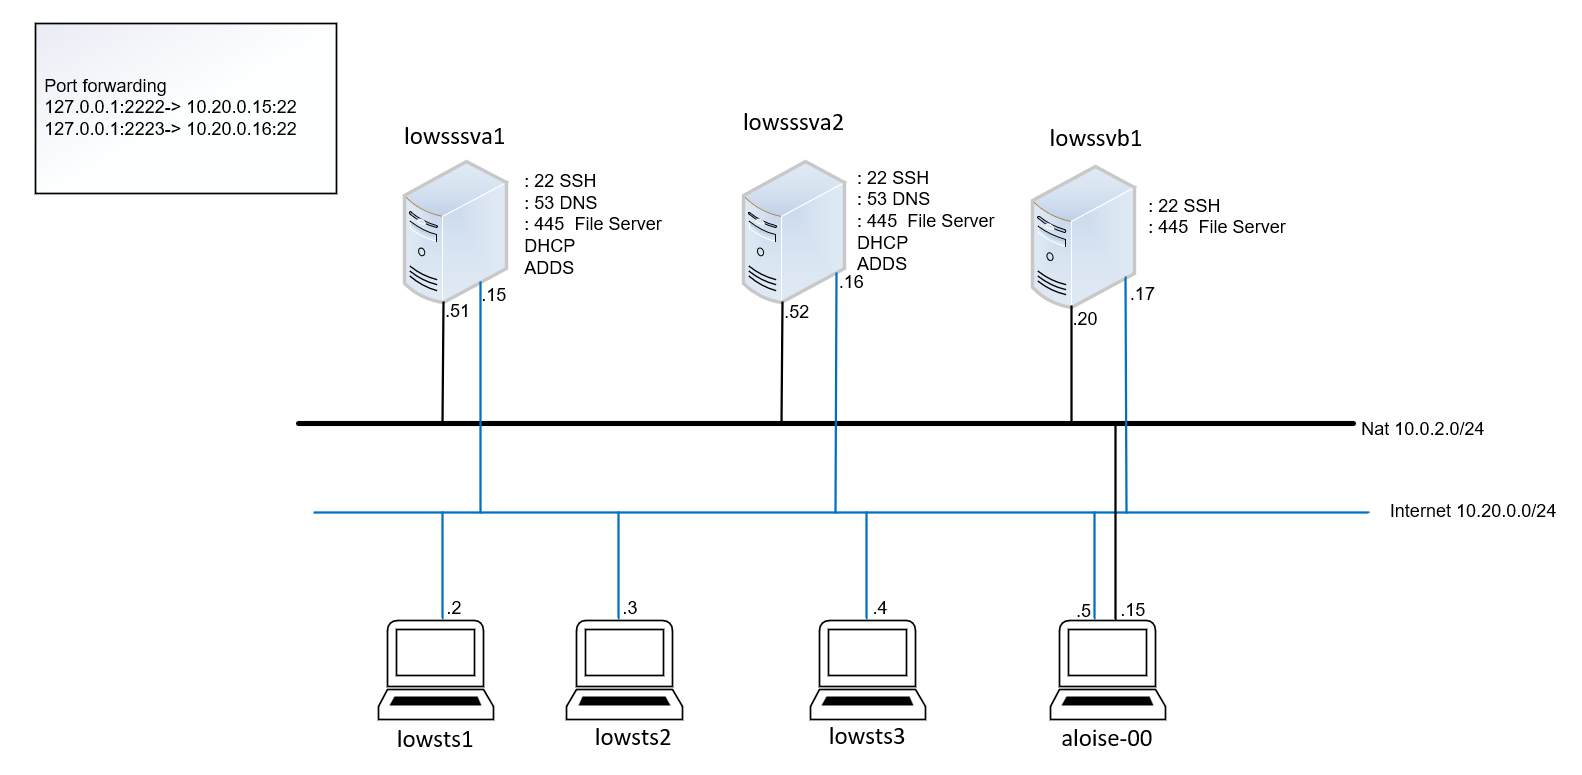
\includegraphics[width=1\textwidth]{Images/schemaRete.PNG}
    \caption{Schema di rete}
\end{figure}

Per questo progetto ho deciso di creare due reti, una NAT e una Interna. Per quanto riguarda la NAT ho deciso di creare la rete 10.0.2.0/24.  Come possiamo vedere i due server che sono in ridondanza tra loro si trovano agli IP 51 e 52 mentre il server FTP a come IP .20. Per quanto riguarda la rete interna ho deciso di darle la 10.20.0.0/24 tutti i pc collegati alla rete ricevono un IP grazie al DHCP mentre i server avranno anche qui un IP fissi come vediamo dallo schema. L'unico pc che è differente sia in nomenclatura che in assegnazioni del IP è il pc del sistemista.


\end{document}  